\begin{pastexam}[label={px:ncku-112-isec-ds-08}]{成大智慧資安學程 112 學年度 第 8 題}
（問答）

(15\%) The following puzzle is called a word ladder: In a word ladder puzzle, you must make the
change occur gradually by changing one letter at a time. At each step you must transform one word
into another word, you are not allowed to transform a word into a non-word. The following sequence
of words shows one possible solution to the problem ``Transform the word ``FOOL'' into the word
``SAGE''.''

\hspace*{1em}Example: FOOL -> POOL -> POLL -> POLE-> PALE -> SALE -> SAGE

Here, we are interested in figuring out the smallest number of transformations needed to turn the
starting word into the ending word.

(a) Construct an example graph by using these words: FOOL, POOL, POLL, POLE, PALE, SALE, SAGE, COOL,
FOUL, FOIL, FAIL, FALL, PALL, POLE, POPE, PAGE. Represent the relationships between the words as a
word ladder graph. (Hint: Think about the path where we get from the word ``FOOL'' to the word
``SAGE'').

(b) Discuss which search algorithm you can use to find an efficient path from the starting word to
the ending word, why it is more efficient compared with other. Discuss the complexity.

(c) There is one way to improve efficiency instead of using a graph to show the relationship.
Suppose that we have a huge number of \textbf{buckets}, each of them with a four-letter word on the
outside, except that one of the letters in the label has been replaced by an underscore. The labels
on the buckets are the keys in our dictionary. The value stored for that key is a list of words.
\textbf{Show the data structure and list the buckets using the following words} (don't list the
buckets containing only one item): FOOL, POOL, POLL, POLE, PALE, SALE, SAGE, COOL, FOUL, FOIL, FAIL,
FALL, PALL, POLE, POPE, PAGE
\end{pastexam}

\begin{pastsoln}
原題的單字表把 POLE 列了兩次，同一個字只當一個頂點，共 $15$ 個字。

\textbf{(a)} 每個字是一個頂點；兩個字只差一個字母（同一位置換一個字母）就連一條無向邊。 逐對比較
$15$ 個字，共得 $19$ 條邊：
\begin{center}
\begin{tabular}{ll}
\toprule
頂點 & 相鄰的字 \\
\midrule
FOOL & POOL, COOL, FOUL, FOIL \\
POOL & FOOL, COOL, POLL \\
COOL & FOOL, POOL \\
FOUL & FOOL, FOIL \\
FOIL & FOOL, FOUL, FAIL \\
FAIL & FOIL, FALL \\
FALL & FAIL, PALL \\
POLL & POOL, POLE, PALL \\
PALL & POLL, FALL, PALE \\
POLE & POLL, PALE, POPE \\
POPE & POLE \\
PALE & POLE, PALL, SALE, PAGE \\
SALE & PALE, SAGE \\
PAGE & PALE, SAGE \\
SAGE & SALE, PAGE \\
\bottomrule
\end{tabular}
\end{center}
畫成圖（粗線是題目範例那條路徑）：
\begin{center}
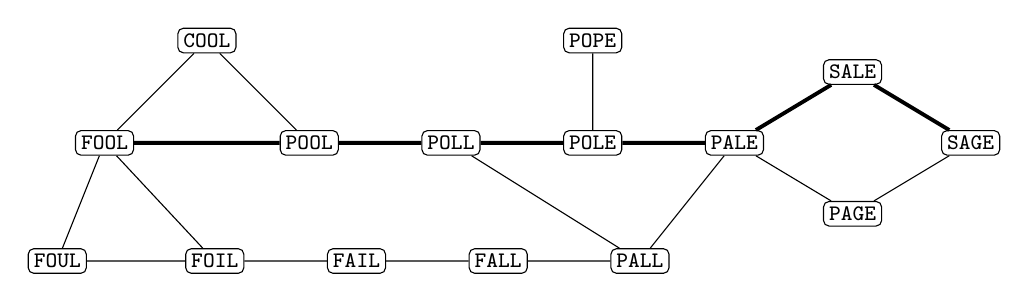
\begin{tikzpicture}[x=1cm,y=1cm,
  w/.style={draw,rounded corners=2pt,inner sep=2pt,font=\footnotesize\ttfamily},
  hl/.style={line width=1.4pt}]
\node[w] (FOOL) at (0,0) {FOOL};
\node[w] (COOL) at (1.3,1.3) {COOL};
\node[w] (POOL) at (2.6,0) {POOL};
\node[w] (FOUL) at (-0.6,-1.5) {FOUL};
\node[w] (FOIL) at (1.4,-1.5) {FOIL};
\node[w] (FAIL) at (3.2,-1.5) {FAIL};
\node[w] (FALL) at (5.0,-1.5) {FALL};
\node[w] (POLL) at (4.4,0) {POLL};
\node[w] (PALL) at (6.8,-1.5) {PALL};
\node[w] (POLE) at (6.2,0) {POLE};
\node[w] (POPE) at (6.2,1.3) {POPE};
\node[w] (PALE) at (8.0,0) {PALE};
\node[w] (SALE) at (9.5,0.9) {SALE};
\node[w] (PAGE) at (9.5,-0.9) {PAGE};
\node[w] (SAGE) at (11.0,0) {SAGE};
\draw (FOOL)--(COOL) (COOL)--(POOL) (FOOL)--(FOUL) (FOOL)--(FOIL) (FOUL)--(FOIL)
      (FOIL)--(FAIL) (FAIL)--(FALL) (FALL)--(PALL) (POLL)--(PALL) (PALL)--(PALE)
      (POLE)--(POPE) (PALE)--(PAGE) (PAGE)--(SAGE);
\draw[hl] (FOOL)--(POOL) (POOL)--(POLL) (POLL)--(POLE) (POLE)--(PALE) (PALE)--(SALE) (SALE)--(SAGE);
\end{tikzpicture}
\end{center}
題目要的是最少的變換次數，也就是圖上 FOOL 到 SAGE 的最短路徑（邊數最少）。 (b) 用 BFS 算出來是
$6$ 次，題目的範例已經是最短的。

\textbf{(b)} 用\textbf{廣度優先搜尋}（BFS，資結書第~21.3~節）。 每一步變換的代價都一樣（無權圖），
BFS 從起點一層一層往外擴：先找出距離 $1$ 的所有字，再找距離 $2$ 的，……。 第一次碰到終點時，
所在的層數就是最少的變換次數（資結書定理~21.4：BFS 求出的 $d[v]$ 就是無權圖的最短距離）。
記下每個字是從誰擴出來的（前驅 $\pi$），從終點沿 $\pi$ 倒回去就是路徑。

從 FOOL 出發，鄰居依字母順序加入佇列：
\begin{center}
\begin{tabular}{lll}
\toprule
取出 & 新發現（距離） & 佇列 \\
\midrule
FOOL & COOL, FOIL, FOUL, POOL（1） & COOL, FOIL, FOUL, POOL \\
COOL & -- & FOIL, FOUL, POOL \\
FOIL & FAIL（2） & FOUL, POOL, FAIL \\
FOUL & -- & POOL, FAIL \\
POOL & POLL（2） & FAIL, POLL \\
FAIL & FALL（3） & POLL, FALL \\
POLL & PALL, POLE（3） & FALL, PALL, POLE \\
FALL & -- & PALL, POLE \\
PALL & PALE（4） & POLE, PALE \\
POLE & POPE（4） & PALE, POPE \\
PALE & PAGE, SALE（5） & POPE, PAGE, SALE \\
POPE & -- & PAGE, SALE \\
PAGE & SAGE（6） & SALE, SAGE \\
\bottomrule
\end{tabular}
\end{center}
SAGE 的距離是 $6$，沿前驅倒回：SAGE $\leftarrow$ PAGE $\leftarrow$ PALE $\leftarrow$ PALL
$\leftarrow$ POLL $\leftarrow$ POOL $\leftarrow$ FOOL，得 FOOL $\to$ POOL $\to$ POLL $\to$ PALL
$\to$ PALE $\to$ PAGE $\to$ SAGE，也是 $6$ 次。 最短的路徑共有 $4$ 條（第 $3$ 步走 POLE 或 PALL、
第 $5$ 步走 SALE 或 PAGE），題目的範例是其中一條；BFS 找到哪一條取決於鄰居的順序，長度一定是 $6$。

為什麼比其他方法好：
\begin{itemize}
\item \textbf{DFS} 沿一條路一直走到底，第一次碰到終點時走的路不一定最短（例如先走 FOIL、FAIL、
FALL、PALL、PALE、\ldots 會繞遠路）。 要保證最短只能把所有路徑都試過，最壞是指數時間。
\item \textbf{Dijkstra} 也能求最短路徑，但它是給有權重的圖用的，要用優先佇列，
$O((|V| + |E|)\lg|V|)$；每條邊權重都是 $1$ 時，BFS 的普通佇列就有同樣的效果，少掉 $\lg$ 的因子。
\end{itemize}

複雜度：圖建好以後，BFS 每個頂點進出佇列一次、每條邊看兩次（無向），時間 $O(|V| + |E|)$，空間
$O(|V|)$（佇列、距離、前驅）。 建圖本身：$n$ 個長度 $L$ 的字兩兩比較，要 $O(n^2 L)$，字典很大時
（例如幾千個四個字母的字）這才是瓶頸，(c) 就是改善這一步。

\textbf{(c)} 資料結構是一個\textbf{字典}（雜湊表，資結書第~12~章）：鍵是把字的某一個位置換成底線
的「桶子標籤」，值是一個串列，存所有符合這個標籤的字。 每個四個字母的字放進 $4$ 個桶子，例如
FOOL 放進 \texttt{\_OOL}、\texttt{F\_OL}、\texttt{FO\_L}、\texttt{FOO\_}。 同一個桶子裡的字彼此只差
那一個位置，兩兩相鄰。 $15$ 個字共產生 $60$ 個（鍵, 字），有兩個字以上的桶子有 $15$ 個：
\begin{center}
\begin{tabular}{ll@{\qquad}ll}
\toprule
鍵 & 值（串列） & 鍵 & 值（串列） \\
\midrule
\texttt{\_OOL} & FOOL, POOL, COOL & \texttt{PA\_E} & PALE, PAGE \\
\texttt{FO\_L} & FOOL, FOUL, FOIL & \texttt{PAL\_} & PALE, PALL \\
\texttt{PO\_L} & POOL, POLL & \texttt{SA\_E} & SALE, SAGE \\
\texttt{P\_LL} & POLL, PALL & \texttt{\_AGE} & SAGE, PAGE \\
\texttt{POL\_} & POLL, POLE & \texttt{F\_IL} & FOIL, FAIL \\
\texttt{P\_LE} & POLE, PALE & \texttt{FA\_L} & FAIL, FALL \\
\texttt{PO\_E} & POLE, POPE & \texttt{\_ALL} & FALL, PALL \\
\texttt{\_ALE} & PALE, SALE & & \\
\bottomrule
\end{tabular}
\end{center}
兩個三個字的桶子各給 $3$ 條邊，十三個兩個字的桶子各給 $1$ 條，共 $3 + 3 + 13 = 19$ 條，和 (a)
的圖一致。 改善的地方：每個字只要算出 $L$ 個鍵、各插入一次，建字典是期望 $O(nL)$ 次雜湊表操作
（每次算鍵、比較鍵花 $O(L)$），不用 $O(n^2)$ 對逐一比較。 BFS 時要找一個字的鄰居，就看它那
$L$ 個桶子裡的其他字；連邊都不必事先建好，直接在字典上跑 BFS 即可。
\end{pastsoln}
